\subsection{PI-Kamera vs. Netzwerkkamera}
Bei Auslösen des System im Überwachungsmodus soll ein aktuelles Bild der  Überwachungs- kamera an das jeweilige Smartphone gepusht werden. Es gibt zwei mögliche Kameratechniken, entweder direkt mit dem Raspberry Pi verbunden oder über das Netzwerk erreichbar.
\paragraph{Raspberry Pi Cam} 
Die Kameras für den Raspberry Pi können direkt an das Gerät angeschlossen werden. Meistens werden sie direkt über Erweiterungsplatinen mit den GPIO Pins verbunden. Der Vorteil dieser Anbindung ist, dass sie keine externe Stromversorgung benötigen und durch viele verschiedene Frameworks leicht ansteuerbar und verwaltbar sind. Der große Nachteil ist allerdings, dass die Kamera direkt an dem Raspberry Pi angeschlossen werden muss. Da dieser möglichst wettergeschützt (im Außenbereich) oder unauffällig (im Innenbereich) angebracht ist, lässt sich von diesen Positionen kaum eine effektive Videoüberwachung realisieren. \\

\paragraph{Netzwerkkamera} 
Eine Netzwerkkamera oder auch IP-Kamera genannt befindet sich im Netzwerk und kann über eine Website oder App eingesehen und gesteuert werden. Der Vorteil ist, dass sie sich an einem beliebigen Ort befinden kann, solange sie im selben Netzwerk ist. Somit kann zum Beispiel eine wetterfeste Kamera im Außenbereich angebracht werden und der Raspberry Pi kann im geschützten Innenbereich stehen. \\
Der Nachteil bei IP-Kameras besteht darin, dass es wenige einheitliche APIs zum Abgreifen des Videomaterials gibt. Die meisten IP-Kameras bieten die Möglichkeit, die Aufgenommenen Bilder auf einem FTP-Server abzulegen. Weiter wäre eine mögliche Lösung das Laden der HTML-Code über einen HTTP-Request und darauffolgend das Ausfiltern des Bildmaterials. Über diese Variante kann kein Video sondern nur statische Bilder geladen werden. Eine weitere Möglichkeit ist das Verwenden eines Videostreams. Dieser könnte mit dem Raspberry Pi ausgewertet und in Bilder umgewandelt werde.
 \\\\
Da in diesem Projekt nicht garantiert ist, dass der Raspberry Pi an einer passenden Position angebracht ist wird für dieses Projekt wird eine IP-Kamera verwendet. Dies trägt außerdem zur universellen Einsatzbarkeit bei.

\subsection{Herangehensweise Ansteuerung}
Aus Recherche und Überlegung haben sich die folgenden Möglichkeiten ergeben:

\paragraph{Auswertung des RTSP-Protokolls mit Python}
Die meisten Netzwerkkameras bieten einen Video-Stream über das Real Time Streaming Protokoll (RTSP) an. Dieser könnte mit Python ausgelesen und interpretiert werden. 

\paragraph{Speicherung des Video-Streams mit FFmpeg}
Außerdem ist es möglich mit dem Tool FFmpeg den Stream auszuwerten und zu bearbeiten.

\paragraph{Speicherung des Bild mittels Screenshot oder HTTP-Request}
Der erste und theoretisch einfachste Ansatz ist die Anfertigung eines Screenshots des Kamerabildes oder das Abrufen des Bildes mit einem HTTP-Request.  

\subsection{Auswertung des RTSP/RTP-Protokolls mit Python}
Das Real-Time-Streaming-Protokoll ist ein Netzwerkprotokoll zur Steuerung von kontinuierlichen Übertragungen in Netzwerken. Dagegen werden über das Real-Time-Prokoll die tatsächlichen Video- und Tondaten übertragen. So werden mit RTSP die Übertragungsdetails festgelegt um im Anschluss mit RTP die tatsächlichen Daten zu übertragen. \\
\paragraph{RTSP Handshake}
Der Handshake zwischen Client und Server basiert auf Strings und ist somit leicht auszuwerten. Zusätzlich ist der Ablauf sehr kurz und übersichtlich gehalten.
Grundsätzlich lässt sich der Handshake in folgende Schritte aufteilen (Server = Kamera):
\begin{enumerate}
	\item Der Client sendet eine Anfrage an den Server. Diese enthält seine IP und den Port.
	\item Als Antwort beschreibt der Server seine Eigenschaften und Funktionen. 
	\item Daraufhin sendet der Client eine Nachricht in der er die Eigenschaften des Streams festlegt (Format, Ports etc).
	\item Der Server bestätigt dies.
	\item Der Client sendet ein 'Play' um die Übertragung zu starten. 
\end{enumerate}
Im Anschluss startet die Übertragung des Streams über RTP.

\subsection{RTSP mit Python}
Eine Mögliche Implementierung des Protokolls in Python hat Sergey Lalov im Jahr 2011 vorgenommen. An diesem Code habe ich Reengineering betrieben. \\
Es wurde ein Server mit dem Twisted Framework implementiert. Dieser empfängt und sendet die Daten der Netzwerkkamera. Das RTSP-Protokoll wird in den einzelnen Schritten abgearbeitet, wobei zu Beginn des Programms die IP, Portbereiche und Userdaten definiert werden. Die einzelnen Protokollschritte werden anhand der 'CSeq' (Identifier für die einzelnen Protokollschritte) identifiziert. Es wird ein Video- und ein Audio-Stream gestartet. Die einzelnen Server-Anfragen sind in Abbildung 4 dargestellt.

\begin{figure}[h]
\begin{minipage}{\textwidth}
	\centering
	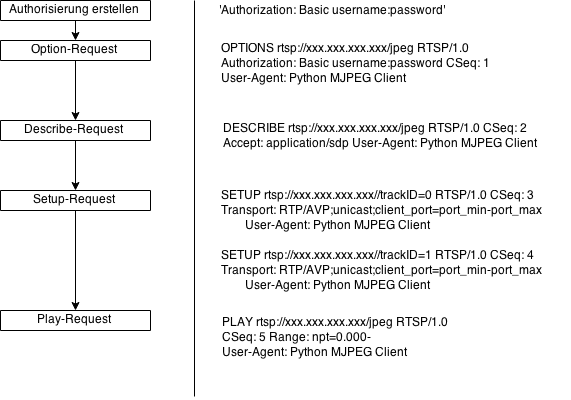
\includegraphics[width=\textwidth]{./data/RTSP.png}
	\caption{RTSP Request-Strings}
\end{minipage}
\end{figure}
\pagebreak

Nach dem PLAY-Request werden zwei neue UDP-Server-Instanzen generiert, die Daten des RTP-Streams auswerten (Audio / Video). Die Implementierung von Sergey Lalov liest an dieser Stelle die einzelnen Bilder eines MJPEG-Stream aus. Bei MJPEG werden in jedem Paket Einzelbilder gesendet. Dies führt dazu, dass aus einem einzelnen Paket ein Bild gewonnen werden kann.  \\
Die Kamera in diesem Projekt hat im RTP-Stream den Videostream im Format H264 ausgegeben. Da dieses Format verschiedene Arten der Komprimierung anwendet, ist nicht in jedem Paket ein einzelnes Bild enthalten. Die Rekonstruktion des Bildmaterials wäre somit sehr aufwändig (keine bestehende Library). \\\\
Die Auswertung des RTP-Streams konnte nicht erfolgreich abgeschlossen werden.  Der Originalcode ist unter Google-Code verfügbar (https://code.google.com/p/python-mjpeg-over-rtsp-client/).


\subsection{Speicherung des Video-Streams mit FFmpeg}
Die Speicherung des Streams ist über eine externe Software möglich. Das Tool FFmpeg ist eine Software-Lösung um Audio- und Videostreams aufzunehmen und zu konvertieren. Es bietet die Möglichkeit, einen Stream aufzuzeichnen und direkt im Anschluss in ein anderes Format zu Wandeln. 
\paragraph{Ablauf}
Im ersten Schritt wird mit FFmpeg der Stream eingelesen und pro Sekunde 3 Bilder daraus erzeugt. 
\begin{lstlisting}[caption = Aufnahme mit FFmpeg, language=python, frame=single, breaklines=true,columns=fullflexible, commentstyle=\color{gray}\upshape, captionpos=b]
ffmpeg -i rtsp://user:pw@$ip:554 -f image2 -vf fps=3 %03d.jpg -loglevel quiet
\end{lstlisting}

Diese Bilder werden in ein Verzeichnis gespeichert. Parallel dazu läuft ein Script, welches alle 60 Sekunden die ältesten Bilder aus diesem Verzeichnis löscht. Dadurch entsteht keine große Datenmenge, es sind nur die aktuellsten Bilder gespeichert. Wenn der Bewegungsmelder auslöst, werden die Bilder aus den letzten 10 Sekunden in ein weiteres Verzeichnis gelegt. Hierauf hat die iOS-App Zugriff über FTP.  \\
\begin{figure}[h]
\begin{minipage}{\textwidth}
	\centering
	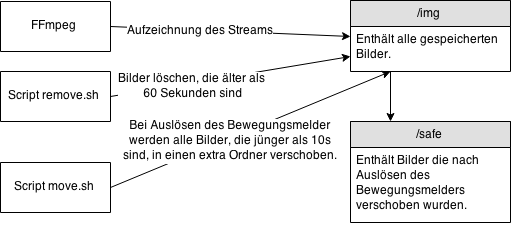
\includegraphics[width=\textwidth]{./data/ffmpeg.png}
	\caption{Ablauf der Aufzeichnung mit FFmpeg}
\end{minipage}
\end{figure}
\paragraph{Vorteil}
Ein großer Vorteil ist die hohe Variabilität der Konvertierung mit FFmpeg. Es kann nahezu jedes Format eingelesen werden und in variablen Frameraten ausgegeben werden. 
\paragraph{Nachteil}
Das Tool FFmpeg erzeugte eine sehr hohe Last auf dem System, da kontinuierlich eine Stream eingelesen wird. 

\subsection{Speicherung des Bild mittels Screenshot}

Ein weiterer Ansatz wäre das Aufrufen der Weboberfläche der Kamera und das Anfertigen eines Screenshots. Dieser könnte abgespeichert und auf einem FTP-Server bereitgestellt werden. \\
Hierfür ist es allerdings erforderlich, dass der Raspberry Pi eine grafische Ausgabe hat. In diesem Projekt soll er nur Serverfunktionalitäten haben. Als Work-Around bietet sich ein virtuelles Display an. Die Virtualisierung kann mittels dem Tool Xvfb realisiert werden. Dieses bietet einen virtuellen Framebuffer, der vom System wie ein normales Display angesprochen werden kann. \\
Die Anfertigung eines Screenshots kann mit dem Tool Selenium erledigt werden. Das Tool Selenium dient zur Automatisierung von Browser-Aktivitäten und wird oft zum Testen von Webanwendungen verwendet. Selenium setzt ein Display vorraus, was durch Xvfb erfüllt wäre. Da Selenium nach Python portiert wurde, könnten die Screenshots direkt aus der Anwendung heraus erstellt werden. \\
Um diese Möglichkeit zu testen, wurde folgender Testcode implementiert:
\begin{lstlisting}[caption = Testcode - Aufnahme Screenshot mit Selenium, language=python, frame=single, breaklines=true,columns=fullflexible, commentstyle=\color{gray}\upshape, captionpos=b, numbers = left]
from selenium import webdriver
import time

start = time.time()
driver = webdriver.Firefox()
driver.get('user:password@ip_of_cam')
// get_screenshot_as_file() gibt das Bild als Binärdaten zurück
img = driver.get_screenshot_as_file()
driver.quit()
end = time.time()
print 'Benötigte Zeit:' + str(start - end)
\end{lstlisting}
Mehrere Messungen haben ergeben, dass das Aufnehmen des Screenshots rund 7 Sekunden dauert. Dies ist auf die geringe Rechenleistung des Raspberry Pi zurückzuführen. Außerdem wird mit Selenium ein vollständiger Browser gestartet, was zu einem enormen Overhead führt. \\
Die Durchführung dieser Methode macht aufgrund der hohen Verzögerung keinen Sinn. Eine Person die den Bewegungssensor auslöst ist längst aus dem Bild verschwunden, bis ein Screenshot aufgezeichnet wird.\\
\subsection{Speicherung des Bild mittels HTTP-Request}

Die nächste Variante ist das Laden des Bildes aus dem HTML-Quelltext der Weboberfläche. Die Analyse des Quelltextes führt schnell zu dem Ergebnis, dass das angezeigte Bild mittels Javascript nachgeladen wird. Mit Python kann ohne weitere Probleme der Quelltext einer Webseite abgerufen werden: 
\begin{lstlisting}[caption = Testcode - Aufnahme Screenshot mit Selenium, language=python, frame=single, breaklines=true,columns=fullflexible, commentstyle=\color{gray}\upshape, captionpos=b, numbers = left]
import urllib2

response = urllib2.urlopen('http://ip_of_cam')
html = response.read()
\end{lstlisting}
Hier offenbart sich direkt das Problem, denn mit der Library urllib2 wird nur der HTML-Code abgerufen, ohne auf die Ausführung von Javascript zu warten. Somit kann über den Code zwar das Image-Objekt identifiziert werden, es enthält allerdings nur das Startbild. Mit dieser Version ist keine Lösung erreichbar. \\
Somit wird ein Framework benötigt, welches zuerst auf die vollständige Ausführen des Javascript-Codes wartet.
\begin{itemize}
	\item \textbf{Selenium}
	Hier könnte ebenfalls wieder Selenium eingesetzt werden, welches einen Export des HTML-Code bietet. Allerdings würde auch hier der Zeitfaktor zu hoch sein. 
	\item \textbf{Scrapy}
	Dies ist ein open-source Framework, mit dem alle Informationen von Webseiten geladen werden könne. Die Installation auf dem Raspberry Pi war nicht erfolgreich.
\end{itemize}
Im nächsten Schritt wurde ein HTTP-Request an die URL gesendet, der im Javascript-Code als erstes aufgerufen wurde. Die Antwort enthielt ein aktuelles Frame der Kamera im Jpeg-Format. Das Abrufen dieses Bildes stellt in den meisten Sprachen keine große Schwierigkeit dar. \\
In Python wird das Bild mit dem Framework Requests und StringIO geladen und in ein Bild umgewandelt. Dieses kann beliebig verarbeitet werden. 
\begin{lstlisting}[caption = Abrufen eines BIldes von einer URL in Python, language=python, frame=single, breaklines=true,columns=fullflexible, commentstyle=\color{gray}\upshape, captionpos=b, numbers = left]
from PIL import Image
import requests
from StringIO import StringIO

r = requests.get('http://user:password@ip:80/tmpfs/auto.jpg')
i = Image.open(StringIO(r.content))
i.save("path/to/safe/python_test.jpg")
\end{lstlisting}
Auch in Swift stellt dies kein Problem dar. Die Daten werden von der URL geladen und in ein UIImage-Objekt gespeichert. 
\begin{lstlisting}[caption = Abrufen eines BIldes von einer URL in Swift, language=c++, frame=single, breaklines=true,columns=fullflexible, commentstyle=\color{gray}\upshape, captionpos=b, numbers = left]
let url = NSURL(string: camurl)
let data = NSData(contentsOfURL: url!)
let image : UIImage! = UIImage(data: data!)
\end{lstlisting}
Im Gegensatz zu der Implementierung mit FFmpeg muss nicht kontinuierlich ein Stream ausgelesen werden, sondern es wird immer nur ein einzelnes Bild ausgelesen, sobald der Bewegungsmelder auslöst. Es lassen sich somit zwei Ansichten realisieren:
\begin{itemize}
	\item \textbf{Archiv:} Bei Auslösen des Bewegungsmelders wird das aktuelle Bild abgerufen und auf einen FTP-Server gespeichert. Die Daten dieses Servers können in der iOS-App unter 'Archiv' abgerufen werden. 
	\item \textbf{Live:} In der iOS-App ist ein Live-View möglich. Dieser liest kein Video-Stream ein, sondern ruft in festgelegten Schritten ein Bild ab und aktualisiert die Ansicht. Um das Bild regelmäßig neu zu laden, wird ein NSTimer genutzt. 
	\begin{lstlisting}[caption = NSTimer in Swift, language=c++, frame=single, breaklines=true,columns=fullflexible, commentstyle=\color{gray}\upshape, captionpos=b]
var timer = NSTimer.scheduledTimerWithTimeInterval(0.5, target: self, selector: Selector("loadImageView"), userInfo: nil, repeats: true)
	\end{lstlisting}
\end{itemize}
\pagebreak
\begin{figure}[h]
	\begin{minipage}{0.9\textwidth}
		\centering
		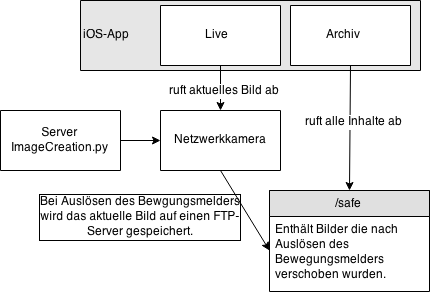
\includegraphics[width=\textwidth]{./data/httprequest.png}
		\caption{Abrufen des Bildes über HTTP-Request}
	\end{minipage}
\end{figure}

\paragraph{Fazit} 
Das Speichern des Kamerabildes mittels Screenshot und RTSP-Protokoll sind fehlgeschlagen. Die Aufnahme mit FFmpeg funktioniert gut, benötigt allerdings sehr viele System-Ressourcen. Somit ist der gewählte Weg in diesem Projekt das Abspeichern des Bildes über einen HTTP-Request. Diese Lösung ist gut in Python und Swift umzusetzen. 

